\chapter{引言}
\label{cha:intro}

\section{超表面的简介及研究现状}
超表面$\left ( \textrm{metasurface} \right )$,是最近提出的一种二维的光学调制器件,具有广泛的应用前景 \cite{intro02}。超表面由三个方向的尺度都小于波长的结构单元组成的阵列(纳米柱)组成,利用超表面不同位置对入射光施加不同程度的调制,通过光的干涉特性,实现特定的出射波前\cite{intro01}。超表面光学器件可以用超薄的表面结构实现传统体结构光学器件的功能,比如起偏器、检偏器、透镜等。超表面的结构示意图如图 ~\ref{fig:c1fig1} \cite{structure} 所示。
\begin{figure}[H] % use float package if you want it here
  \centering
  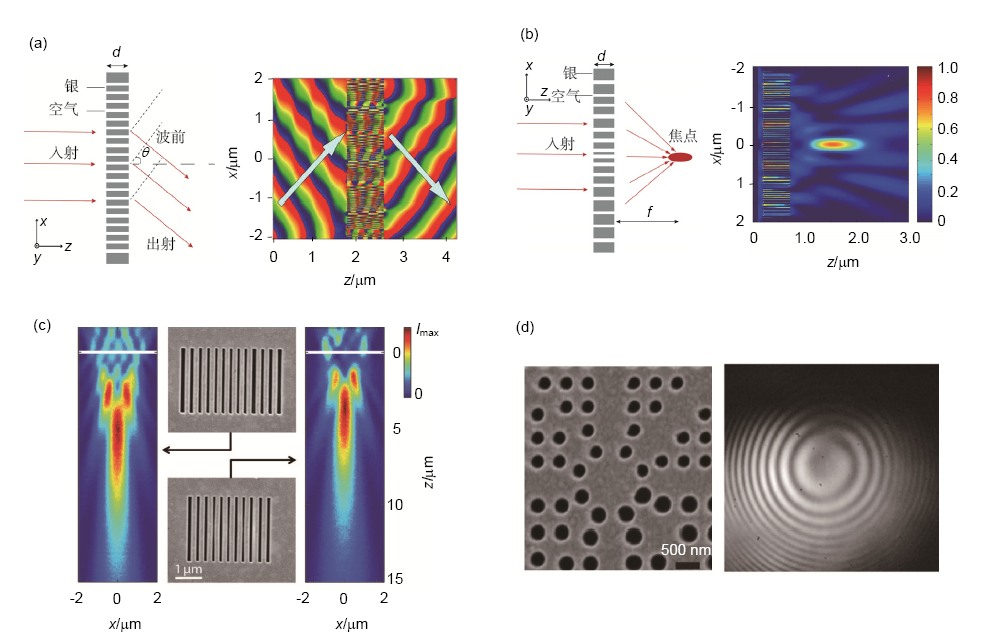
\includegraphics[width=\textwidth]{metasurfaceintro.png}
  \caption{超表面的结构示意图}  \cite{intro01}
  \label{fig:c1fig1}
\end{figure}

尽管超表面目前的具有喜人的应用前景,但是文献调研结果表明,目前的超表面存在一个明显的问题,即超表面一旦被制作出来,它的光学性质就是固定的。这样,对于不同的光学需求而言就需要根据具体问题进行不同的超表面的制备。为此,寻求一种能够在不改变超表面光学器件结构的情况下而能够根据需要改变其光学特性的方法具有重要的实用价值。

\begin{figure}[H] % use float package if you want it here
  \centering
  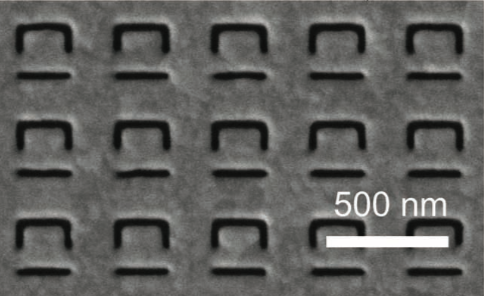
\includegraphics{planestr.png}
  \caption{超表面的周期化二维结构}
  \label{fig:c1fig1}
\end{figure}


\section{GST简介}
\label{sec:first}

GST材料作为一种相变材料,目前已经被广泛应用在光学存储设备中,诸如DVD, CD-ROM中 \cite{savemedia} \cite{tbt}。有关GST材料在存储材料应用场合的挖掘是目前的研究热点之一。GST材料在不同条件下可以实现晶态结构和非晶态结构之间的转化。目前常见的变换晶相结构的方式有两种:热退火和电脉冲,而激光控制GST相变 \cite{laser} 的原理同热退火一致。其中,Ge$_{2}$Sb$_{2}$Te$_{5}$材料在$300 ^{\circ}$C左右退火可以实现从非晶态到晶态到转化,而从$600^{\circ}$C快速退火时可以从晶态转化为非晶态 \cite{GSTbase} 。图 ~\ref{fig:annealing} 展示了退火导致相变的简要过程。

\begin{figure}[H] % use float package if you want it her e
  \centering
  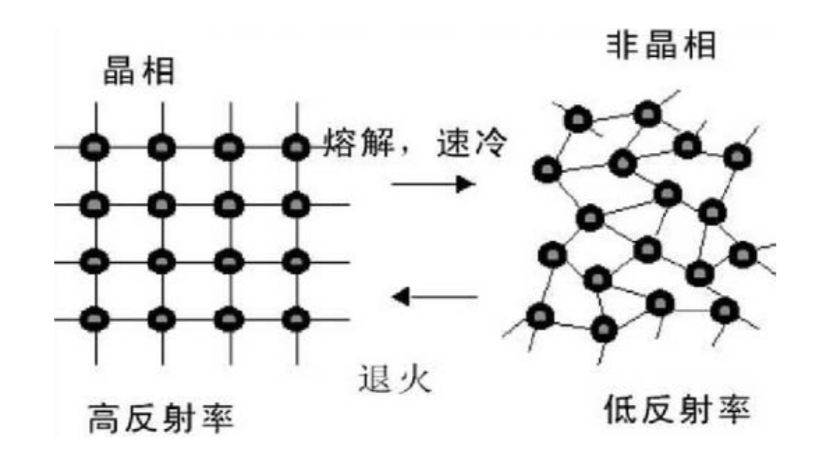
\includegraphics{annealing.png}
  \caption{退火导致相变的简要过程} \cite{GSTbase2}
  \label{fig:annealing}
\end{figure}

同时,GST材料的相变过程也可以通过施加电脉冲来实现。文献 \cite{elePhaseChange} 指出,对于$Ge_{2}Sb_{2}Te_{5}$而言,施加一个短而电压稍高的脉冲(文献中给出的是$\left (6V - 100\ ns \right )$)可以使得GST材料实现从晶态到非晶态的转变;而对于与之相反的过程,文献中给出的电压脉冲形式是$\left (4V - 500\ ns \right )$。如图 ~\ref{fig:elephaseChange} 所示,GST的电特性在相变数十万次之后才会发生显著改变。
\begin{figure}[H] % use float package if you want it here
  \centering
  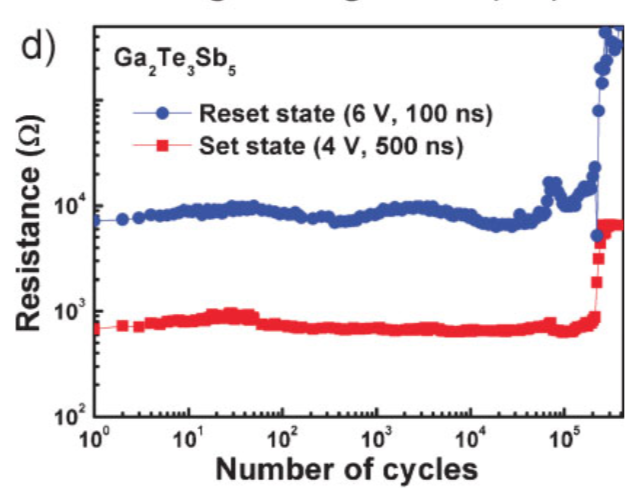
\includegraphics[width = 0.6\textwidth]{elePhaseChange.png}
  \caption{GST材料经过电控的相变过程后电阻的变化} \cite{elePhaseChange2}
  \label{fig:elephaseChange}
\end{figure}

GST本身相变的时间很短,只有纳秒量级 \cite{fast}。如果采用热退火的话,升温和冷却的过程会将这个很短的相变时间淹没,从而难以体现迅速相变的优势;而由于电脉冲诱导GST相变仅需数百纳秒,这可以实现存在相变需求时的快速调节。同时,由于实现纳米尺度的隔热相对困难,而类似尺寸的电极较为易于实现;因此电脉冲控制会更容易实现对GST结晶状态的精确控制。为了实现对各个位置的纳米柱都能进行电位控制,同时又不影响材料的光学特性;我们决定采取ITO-GST-ITO的三层结构,其中ITO为一种透光率高于90\% 的导电材料,是现在应用面比较广的透明电极材料。下图为为了实现对每个纳米柱的控制,我们可以采取的电极排布与加工方法:
\begin{figure}[H] % use float package if you want it here
  \centering
  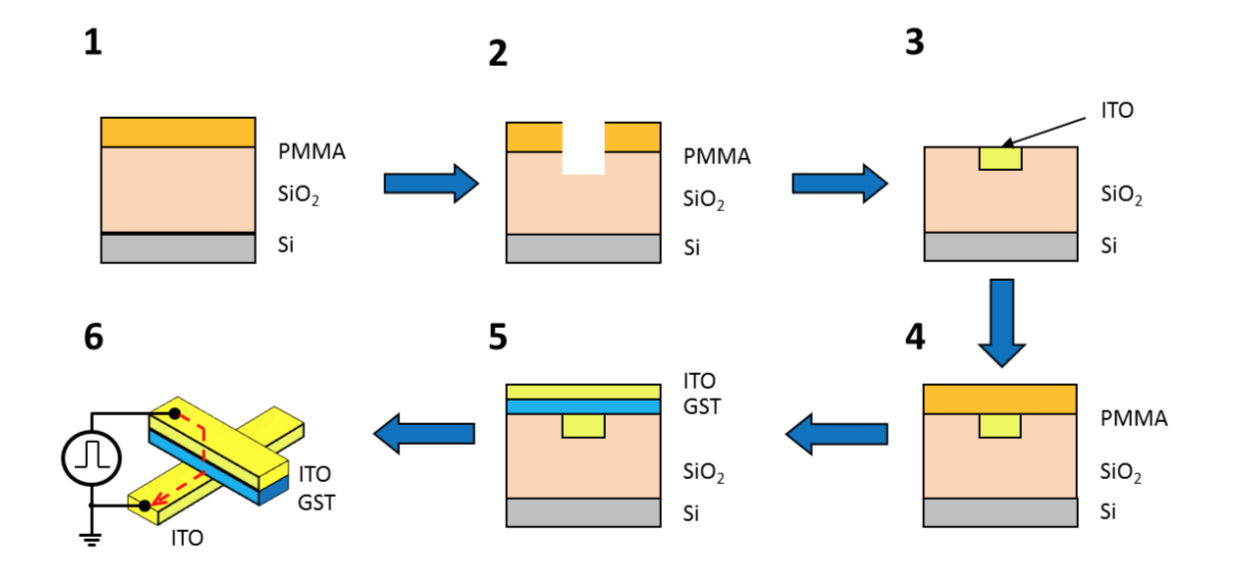
\includegraphics[width = 0.8\textwidth]{itogstito.png}
  \caption{制作三层电极结构的主要过程。}
  \label{fig:elephaseChange1}
\end{figure}

上图展示了制作三层电极结构对主要流程。1. PMMA溅射到了SiO$_{2}$衬底上,并形成一维结构。2. 在氩气氛围下刻出沟槽。3. 在沟槽中以ITO填充,并洗掉表面的PMMA。 4. 生长一层新的PMMA。 5. 按照PMMA形成的一维结构依次溅射GST和ITO。 6. 将三层结构抬离SiO$_{2}$,形成条状电极结构。

Ge$_{2}$Sb$_{2}$Te$_{5}$材料在相变前后折射率的显著差异可以用于制备光学特性可变的超表面光学器件\cite{refocus}。简而言之就是使用GST材料制备超表面中的纳米柱,并通过改变不同位置的纳米柱晶化状态来改变超表面的光学特性。根据文献调研 \cite{GSTnk} 和后续采用椭圆偏振仪测得的结果来看,GST在非晶态时的折射率约为$\left (4 + 0.5i \right )$,而晶化之后的折射率约为$\left (6 + 3i \right )$。作为一种相变材料,GST材料具有相变时间短(150$\ $ns)、相变前后结构确定性好、可循环想变次数多(数十万次)的优点 \cite{GSTbase},因此本论文奖探索利用GST材料来制备可控的超表面的方法。

\begin{figure}[H] % use float package if you want it here
  \centering
  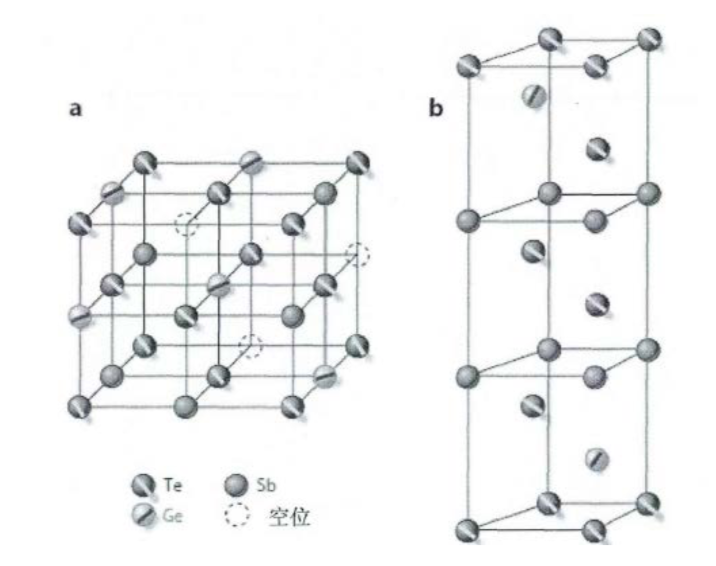
\includegraphics{crystalGST.png}
  \caption{GST材料的两种不同晶化状态} \cite{intro01}
  \label{fig:cGST}
\end{figure}

但是,由于GST材料在晶化与非晶化之间的中间状态尚不明确 \cite{nature},因此本论文将这种材料视为一种具有两种光学特性的材料。为了制作可调超表面光学器件,有两种方式可以考量:
  \begin{itemize}
    \item[-] 强度控制方法:能够有效控制不同位置的、足够大的光强变化;
    \item[-] 相位控制方法: 能够让单个结构单元实现$\left (0, 2\pi \right )$内的相位调节。
  \end{itemize}
目前,对强度调节研究比较好的成果是在1.55 $\mu$m处实现了30 dB的强度隔离\cite{isolation},但这篇文献中实现的是对平面整体的调控而不能实现对平面上各个点的调节。同时,相位控制方法相比于强度控制方法而言,单元尺寸更小,结构可扩展性更好。基于上述原因,我们将后续仿真工作集中在了相位调节上。

\section{实验方法简要说明}
\label{sec:third}
\subsection{GST制备方法}
为了研究GST的相变过程以及光学特性,本论文采用磁控溅射的方法来制备纳米厚度的GST薄膜。磁控溅射指的是在高真空的环境中通入惰性气体,并令惰性气体的离子轰击靶材,使得靶材原子带电并逃逸到空间中,而后在电场作用下 附着到样品上从而实现镀膜的过程\cite{sputtering}。 磁控溅射镀膜的方式具有溅射速率稳定、膜组分稳定性好、重复实验过程之间溅射效果一致性好等特点。图 ~\ref{fig:sputtering} 是磁控溅射的简要原理示意图。
\begin{figure}[H] % use float package if you want it here
  \centering
  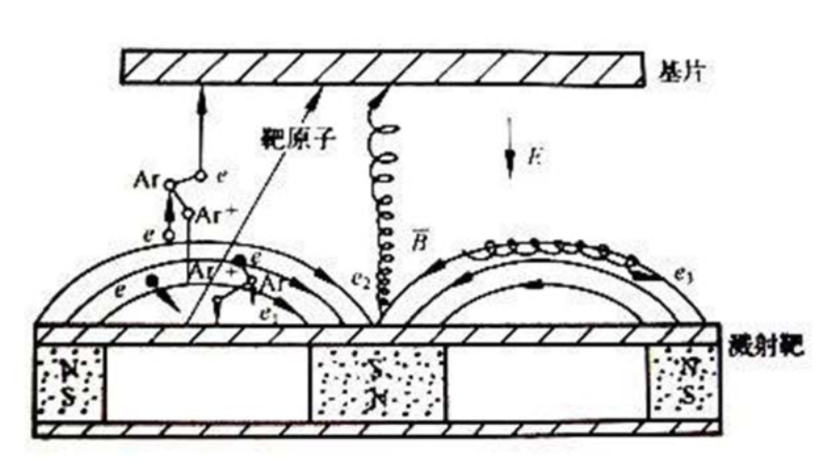
\includegraphics{sputtering.png}
  \caption{磁控溅射原理示意图}\cite{sputtering}
  \label{fig:sputtering}
\end{figure}

与溅射镀膜的质量有关的因素很多,比如溅射的方式、氩气氛围的气压、溅射功率、时间,以及溅射过程中样品是否加热等,而GST材料目前的相关文献非常贫瘠,因此本论文将探索适宜GST的溅射条件。由于GST材料本身的电阻率较高$\left ( >1 k \Omega \cdot{} m \right )$ \cite{ohmofGST},而直流溅射仅适用于导体靶材的溅射。出于对靶材和电极保护的考量,实验过程中仅考虑射频溅射。

\subsection{GST相变方法研究}
本论文用快速退火(RTA)来实现对GST材料的晶化状态的改变。快速退火在氮气氛围下进行,其的目的是防止样片在接近$600\ ^{\circ}$C的温度下受到氧化。根据文献\cite{annealing}调研结果,对于GST材料,无论是晶化过程还是非晶化过程,所需要的退火温度均不超过$500\ ^{\circ}$C。为了防止实验过程中不可避免的样片接触空气对样片造成氧化,我们在退火之前会通5$\ $min $N_{2}$,退火之后会等到反应处冷却至$60\ ^ \circ{} C$以下再取样。但是这并不能彻底杜绝氧化的可能,这点会在后文中展开说明。

\subsection{GST复折射率研究}
本论文使用椭偏仪来对GST的复折射率和厚度进行测量。由于椭偏仪仿真时间过长,因此在本次研究中采用台阶仪来获得样品厚度的数据。(有关其原理详见第 ~\ref{subsection:stage} 小节)
椭圆偏振仪的光路示意图如图 ~\ref{fig:oval} 所示:
\begin{figure}[H] % use float package if you want it here
  \centering
  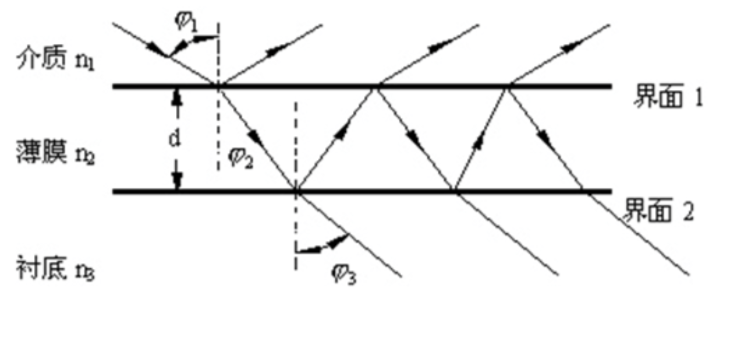
\includegraphics{oval.png}
  \caption{椭圆偏振仪光路示意图}
  \label{fig:oval}
\end{figure}
出射光的波矢与入射波矢之间满足如下方程:
\begin{equation}
G = \frac{E_{rp}}{E_{rs}} \cdot{} \frac{E_{ip}}{E_{is}} = \tan{\Psi \cdot{} e^{i \Delta}} = \frac{r_{1p}+r_{2p}e^{-2i \phi}}{1 + r_{1p}r_{2p}e^{-2i \delta}} \cdot{} \frac{r_{1s}+r_{2s}e^{-2i \phi}}{1 + r_{1s}r_{2s}e^{-2i \delta}}
\end{equation}
其中,$\delta$表示的是膜厚导致的相位差,并满足$\delta = 2 \pi dn_{2} \cos{\phi_{2}} / \lambda$. 椭偏仪通过测量$E_{ip}, E_{is}, E_{rp}, E_{rs}$来拟合薄膜的复折射率和薄膜厚度\footnote{薄膜厚度主要参考台阶仪的测量结果}。
实际上在测量拟合材料的复折射率和厚度中,由于拟合的参数较多,因此容易收敛到一个极值,而这个极值所表征的$\tan{\Psi \cdot{} e^{i \Delta}}$与测量值不符。这种时候需要重新调整拟合中各个参数的初值比较繁琐,因此尽量采用其它途径测量得到与薄膜的复折射率不直接相关的各个参数。

\subsection{GST薄膜光谱透射率和反射率研究}
本论文采用傅立叶光谱仪对GST薄膜对不同波长的光的透过率和反射率进行研究。
傅立叶光谱仪的光学核心是迈克尔逊干涉仪,基本原理是一束光经过分束器之后在待测样品片表面发生干涉,通过测量干涉得到的光强来计算出样品本身的透射率或者反射率,如图 ~\ref{fig:fourier} 所示。
\begin{figure}[H] % use float package if you want it here
  \centering
  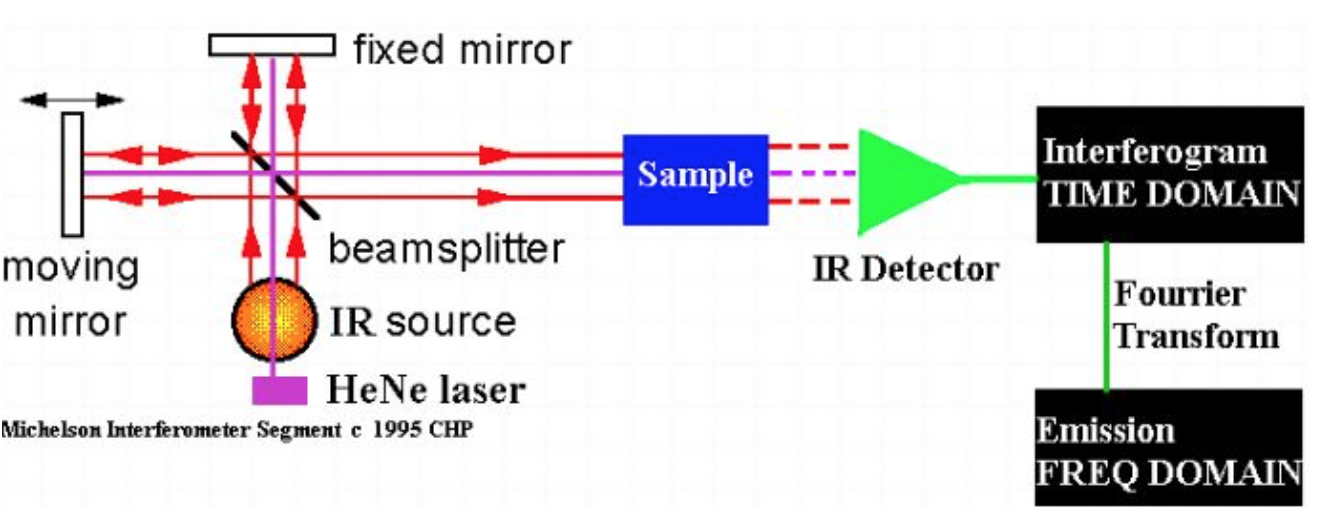
\includegraphics[width=0.8\textwidth]{fourier.png}
  \caption{傅立叶光谱仪原理图}
  \label{fig:fourier}
\end{figure}
和传统的光谱仪相比,傅立叶光谱仪测量的是时域的光强,然后进行傅立叶变换得到频域上的信息,因此具有测量速度快、波数分辨率高的优点。在本项目中,我们为了调查GST材料的光学特性,将这种材料溅射到了铝衬底或者玻璃衬底上,分别得到其反射与透射特性。进而,我们能够从反射特性和透射特性反演出材料的复折射率,与用椭偏仪测定的数据进行对比,从而判断试验结果产生的误差主要来源。

\section{本文结构安排}
本文围绕GST的光学特性进行展开,具体包括优化的超表面的结构,对GST磁控溅射条件的优化,以及对GST薄膜的光学特性研究和结构组分研究。

本论文按照以下方式进行展开:本章主要介绍课题的研究背景,包括超表面的研究现状、GST材料的特性以及实验方法。

第二章介绍了基于FDTD的仿真结果,与优化的超表面结构。

第三章介绍了GST薄膜的制备和光学特性、组分特性的研究。

第四章对本次项目进行总结,并提出了后续的研究思路。